%%%%%%%%%%%%%%%%%%%%%%%%%%%%%%%%%%%%%%%%%%%%%%%%%%%%%%%%%%%%%%%%%%%%%%%%%%%%%%%%
%2345678901234567890123456789012345678901234567890123456789012345678901234567890
% 1 2 3 4 5 6 7 8

\documentclass[letterpaper, 10 pt, conference]{ieeeconf} % Comment this line out if you need a4paper

%\documentclass[a4paper, 10pt, conference]{ieeeconf} % Use this line for a4 paper

%\IEEEoverridecommandlockouts % This command is only needed if 
     % you want to use the \thanks command

%\overrideIEEEmargins % Needed to meet printer requirements.

% See the \addtolength command later in the file to balance the column lengths
% on the last page of the document

% The following packages can be found on http:\\www.ctan.org
%\usepackage{graphics} % for pdf, bitmapped graphics files
%\usepackage{epsfig} % for postscript graphics files
%\usepackage{mathptmx} % assumes new font selection scheme installed
%\usepackage{times} % assumes new font selection scheme installed
\usepackage{amsmath} % assumes amsmath package installed
\usepackage{amssymb} % assumes amsmath package installed
\usepackage{graphicx}
\usepackage{tabularx}

\title{\LARGE \bf
Sandhi: An open source alternative to LabVIEW
}


\author{Albert Author$^{1}$ and Bernard D. Researcher$^{2}$% <-this % stops a space
\thanks{*This work was not supported by any organization}% <-this % stops a space
\thanks{$^{1}$Albert Author is with Faculty of Electrical Engineering, Mathematics and Computer Science,
     University of Twente, 7500 AE Enschede, The Netherlands
     {\tt\small albert.author@papercept.net}}%
\thanks{$^{2}$Bernard D. Researcheris with the Department of Electrical Engineering, Wright State University,
     Dayton, OH 45435, USA
     {\tt\small b.d.researcher@ieee.org}}%
}


\begin{document}



\maketitle
\thispagestyle{empty}
\pagestyle{empty}


%%%%%%%%%%%%%%%%%%%%%%%%%%%%%%%%%%%%%%%%%%%%%%%%%%%%%%%%%%%%%%%%%%%%%%%%%%%%%%%%
\begin{abstract}

This paper is an attempt to lay down a software framework for systematic development of an open source functional clone to LabVIEW. It has been named Sandhi ("to connect" in Sanskrit) and it has been developed to serve as visual programming tool for control system applications.

\end{abstract}


%%%%%%%%%%%%%%%%%%%%%%%%%%%%%%%%%%%%%%%%%%%%%%%%%%%%%%%%%%%%%%%%%%%%%%%%%%%%%%%%
\section{INTRODUCTION}
Visual programming languages like LabVIEW are important and required as they cut short the time of prototyping a control algorithm and thereby giving the control scientists and engineers freedom to test their control heuristics. The problem with tools like LabVIEW is their proprietary nature.
A proprietary software has inherent limitations as they can't be embraced by one and all in the same manner. This paper exposes the development of Sandhi an open source alternative to LabVIEW. This is an important software project under the aegis of FOSSEE initiative at IIT Bombay. The FOSSEE initiative focuses on development of open source software primarily for use by academia.


\section{SANDHI}
\subsection{Overview}

Sandhi is aimed at becoming a visual programming tool for replacing LabVIEW. It's current form is raw, however if the control community gets excited by this tool, this tool can achieve a lot of what LabVIEW can do. The release of the $\beta$ version of Sandhi is under way.

It has been named Sandhi as it means connecting and conveys our idea of connecting various blocks to come up with a robust visual program.

Sandhi is a pure python implementation using the GNU Radio's framework. It reaps advantage of Scilab's computational engine via sciscipy. Sciscipy is an Application Programming Interface aimed at Inter Process Communication with Scilab, when in the workspace of Python programming language.

The implementation of feedback was achieved by using a new application scheduler written specifically for this purpose. GRAS stands for GNU Radio Advanced Scheduler, it has been used in all the developments. It was impossible to implement the feedback with the stock application scheduler. Application Scheduler is responsible for threading, controlling the data flow and managing the use of the computer resources like processor time to various processes.


\subsection{Scope}
Sandhi as aforementioned, uses GNU Radio at its core. GNU-Radio was identified as a very promising Data Acquisition(DAQ) tool, and hence Sandhi inherits following advantages-

\begin{itemize}
\item It has a massive device driver library, thereby it supports a good range of DAQ cards from GNU Radio's UHD(Universal Software Radio Peripheral Hardware Driver) module and Comedi(data library based on Linux Kernel Drivers).
\item Clean GUI; various widgets that can be used to tweak the inputs in real time like sliders, knobs etc.
\item Possible to implement blocks entirely in python as well as C++
\item Real time response to changes in calculation parameters, benefit of using C++ compiled binaries.
\end{itemize}

We could make GNU Radio interact with Scilab�s computation engine, allow feedback loop which was not tried earlier. This could work as a potential replacement to LabVIEW.


\subsection{Simulation Capabilities}
The functions chosen to illustrate Sandhi�s simulation capabilities are following:
\begin{itemize}
\item csim - used for generating continuous time response of linear systems.
\item dsim - used for generating discrete time response of linear systems.
\end{itemize}
The following screenshots demonstrate simulations in Sandhi

\begin{figure}[ht!]
	\centering
	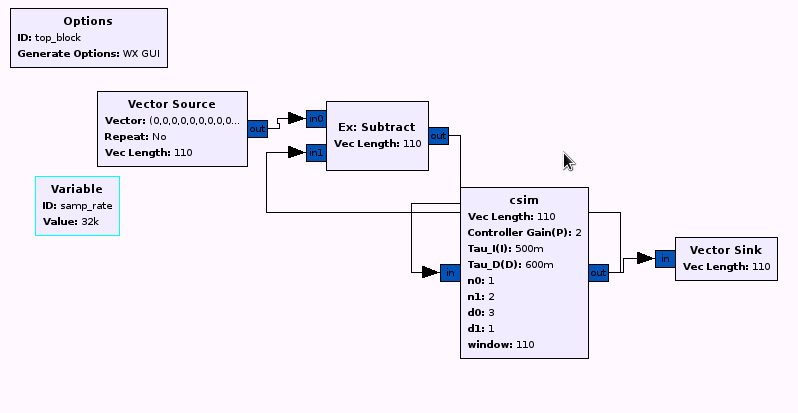
\includegraphics[width=90mm]{csim.png}
	\caption{Continuous time simulation flowgraph}
	\label{overflow}
\end{figure}

\begin{figure}[ht!]
	\centering
	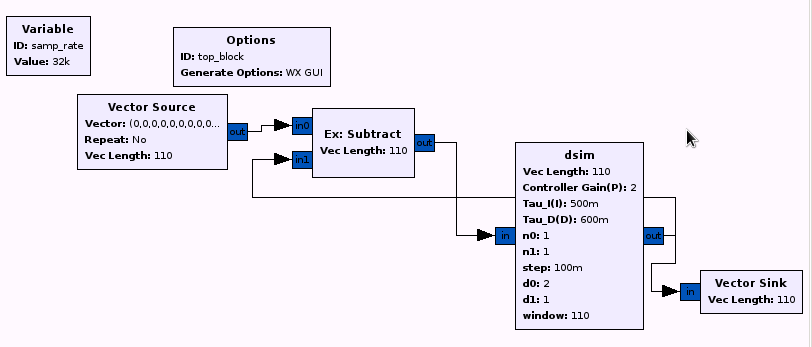
\includegraphics[width=90mm]{dsim.png}
	\caption{Discrete time simulation flowgraph}
	\label{overflow}
\end{figure}


\begin{figure}[ht!]
	\centering
	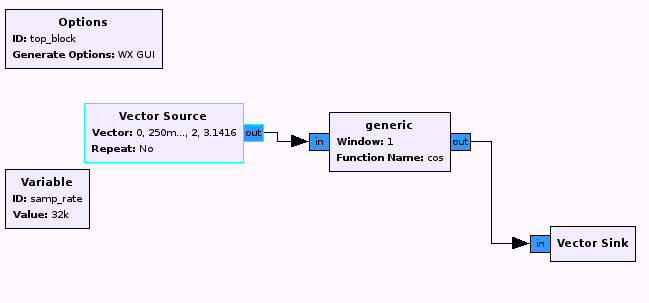
\includegraphics[width=90mm]{generic_block.png}
	\caption{A scilab generic block calling cosine function from scilab's computational engine}
	\label{overflow}
\end{figure}


\subsection{Plant-Controller Block}
SBHS or Single Board Heater System is a small portable plant with time response of around 30 seconds developed at IIT Bombay. One can perform open loop tests as well as closed loop tests on SBHS. SBHS uses ATMega16 microcontroller for communication as well as control of the plant. It can be connected to any standard USB port of Laptop or PC using serial RS232 protocol. SBHS has 3 variables, temperature being a controlled variable and heater and fan (rpm) values being manipulated variables.

So far we've been able to solve the servo problem using Sandhi. The work on regulatory problem is under-way. The controller controls the plant as per the backward difference equation 
\begin{equation}
	\begin{split}
	u(t) =u(t-1) + K_c[e(t)-e(t-1)] +  {\frac{K_c T_s}{T_i}}e(t) + \\
	{\frac{K_c T_d}{T_s}}[e(t)-2e(t-1)+e(t-2)] 
	\end{split}
\end{equation}

The backward difference equation approximation requires one to deal with previous time instances (for example: (t-1)\textsuperscript{th} instant). Sandhi internally uses FIFO Queue implementation to deal with this. We reutilize an existing python data structure called list to implement FIFO Queue. Implementation of FIFO queue in Sandhi is in two steps-

\begin{enumerate}
	\item We initialize queue with fixed queue length and each element with zero value. The queue length is determined by number of past time instances required in backward difference equation approximation. For our case, we require time instances up to (t-2); so the queue length will be of 3 elements namely for input at $t = t$, $t = t-1$, $t = t-2$. We also initialize a \verb|t_1| variable for (t-1)\textsuperscript{th} instance as 0.

	\item Work function of gr-controller script of Sandhi runs several times for each input. Queue structure on first run of work function:

	\begin{itemize}
		\item  {[}0, t-1, t{]}
 		where 't' is input of that time instance
		\item {[}t(N-2), t(N-1), t(N){] queue structure after N\textsuperscript{th} time instant }
		\item we pop the queue completely in variables and then use them in backward difference equation.
	\end{itemize}
\end{enumerate}

But all of this is abstracted to the user, and he/she has to care only about the variables, controller parameters, and their flow. Set point tracking demonstrated using SBHS Plant-Controller blocks in Sandhi.

\begin{figure}[ht!]
	\centering
	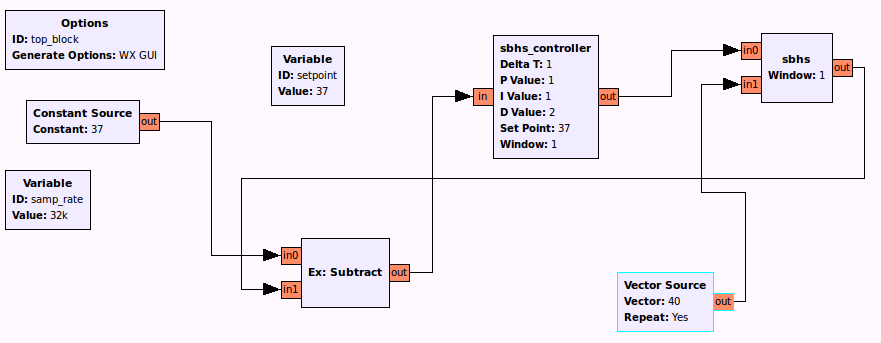
\includegraphics[width=90mm]{sbhs_sandhi.png}
	\caption{Set point tracking of SBHS in Sandhi}
	\label{overflow}
\end{figure}


\section{Porting it onto Aakash}
Aakash is a low cost android-based tablet promoted by Indian Government, and distributed to technical colleges and universities primarily to enhance e-learning. Aakash is built on Allwinner Sun5i platform and hence runs Ubuntu-for-ARM GNU/Linux operating system by booting the image from SD card.
Sandhi needs to be compiled again on Aakash with all its dependencies which are available in central repositories. It is necessary that a memory swap space (at least 512mb) be enabled for software to compile properly. Compilation procedure is standard and it takes around 8 hours to complete.
Sandhi runs smoothly on Aakash since it has minimum runtime requirements. Using USB multi-port hubs, it is possible to run SBHS(Single Board Heater System) similarly as one would do on standard GNU/Linux system.

\section{CONCLUSIONS}

LabVIEW has a great legacy and a lot of development and support has given by National Instruments. However for academic institutions and for educational purposes, a free and open source software is essential and Sandhi is an attempt to fill this void. Sandhi primarily focuses on control system applications but its framework is ready to extend it to newer paradigms. With its access to Scilab's rich computational engine, Sandhi can be extended from simple image processing filter blocks to complex backward propogation of neural networks. Keeping it open and free is necessary for community based development, software code quality, and enhanced learning.

\addtolength{\textheight}{-12cm} % This command serves to balance the column lengths
     % on the last page of the document manually. It shortens
     % the textheight of the last page by a suitable amount.
     % This command does not take effect until the next page
     % so it should come on the page before the last. Make
     % sure that you do not shorten the textheight too much.

%%%%%%%%%%%%%%%%%%%%%%%%%%%%%%%%%%%%%%%%%%%%%%%%%%%%%%%%%%%%%%%%%%%%%%%%%%%%%%%%



%%%%%%%%%%%%%%%%%%%%%%%%%%%%%%%%%%%%%%%%%%%%%%%%%%%%%%%%%%%%%%%%%%%%%%%%%%%%%%%%



%%%%%%%%%%%%%%%%%%%%%%%%%%%%%%%%%%%%%%%%%%%%%%%%%%%%%%%%%%%%%%%%%%%%%%%%%%%%%%%%
\section*{APPENDIX}
\subsection{Source Code for Sciscipy wrapper}
The modified code with an automated builder/installer script especially for Sandhi, is hosted at-
\par \textit{https://github.com/manojgudi/sciscipy-1.0.0}

\subsection{Source Code for Sandhi}
Complete source Code and building instructions are available at-
\par\textit{https://github.com/manojgudi/sandhi}

\subsection{Ubuntu GNU/Linux Images for Aakash tablet}
Getting Ubuntu images for Aakash tablet and instructions for setting it up is provided on-
\par \textit{https://github.com/androportal/linux-on-aakash}

\section*{ACKNOWLEDGMENT}

We'd like to thank the Department of Chemical Engineering and the FOSSEE Group, IIT Bombay for providing us with the resources. We would especially like to thank Professor Kannan Moudgalya, IIT Bombay and Josh Blum for their guidance and support for the project development.

\begin{thebibliography}{99}

	\bibitem{c1} GNU Radio- The Free \& Open Software Radio Ecosystem- Blocks Coding guide in C++ and tutorials for writing Python Application http://gnuradio.org/redmine/projects/gnuradio/wiki/BlocksCodingGuide
	\bibitem{c2} Virtual Labs initiative http://en.wikipedia.org/wiki/Virtual\_Labs\_(India) 
	\bibitem{c3} Inderpreet Arora, Kannan M. Moudgalya, Kaushik Venkata, Victor Chakraborty, Rupak Rokade and Rakhi R., A Low Cost, Scalable, Virtual Control Laboratory, Santiago, Chile, IEEE Conference on Control and Automation.
	\bibitem{c4} Sciscipy: Scilab API for Python http://forge.scilab.org/index.php/p/sciscipy
	\bibitem{c5} Linux on Aakash tablet https://github.com/androportal/linux-on-aakash
	\bibitem{c6} GNU Radio Advanced Scheduler, developed by Josh Blum, Ettus Resarch, https://github.com/guruofquality/gras
	\bibitem{c7} GNU Radio Python blocks Writing python blocks https://github.com/aviralchandra/gr-py\_block
	\bibitem{c8} Jagdish Y. Patil, Balashish Dubey, Kannan M. Moudgalya, Rakesh Peter: GNURadio, Scilab, Xcos and COMEDI for Data Acquisition and Control: An Open Source Alternative to LabVIEW, Article, IIT Bombay, Mumbai 400076
	\bibitem{c9} Dictino Chaos1;*, Jes  �us Chac �on1, Jose Antonio Lopez-Orozco2 and Sebasti �an Dormido1 : Virtual and Remote Robotic Laboratory Using EJS, MATLAB and LabVIEW
	\bibitem{c10} Kannan M. Moudgalya. Digital Control. John Wiley and Sons, 2009
	\bibitem{c11} Scilab, open source software for numerical computation, www.scilab.org
\end{thebibliography}




\end{document}
